% ============================================================
\newpage
\section{Results}\label{sec:results}

The Results section presents the empirical findings of the study.
Results are reported objectively, without interpretation,
and follow the same logical order as the stated objectives and methods.

\lightbadexample{
\textbf{Bad subsection titles}

-- Model performance \\
-- Experimental results \\
-- Evaluation \\
-- Analysis
}

% ============================================================
\subsection{RAG retrieval and prompt engineering yield comparable output quality}

This subsection addresses the evaluation question of whether retrieval-augmented generation provided meaningful improvements over optimized prompt engineering alone.

The system was evaluated in two configurations: (1) a RAG-based approach using semantic retrieval from the indexed knowledge base, and (2) a prompt engineering approach incorporating all toolkit content directly in the system prompt. Both configurations were tested against identical clinical scenarios by the Ariadne Labs technical team and clinician reviewers. Evaluations were conducted both on synthetic clinical scenarios for controlled comparison and during real patient consultations at clinicians' weekly meetings.

Clinician and technical reviewers assessed responses across four dimensions: relevance, clinical tone, actionability, and safety. Neither approach consistently outperformed the other in qualitative assessments. Output differences were not perceptible to reviewers, who rated both configurations as equally appropriate for clinical communication guidance.

Token consumption analysis revealed that the RAG approach consumed approximately 50\% fewer tokens per query on average compared to the prompt engineering approach, which incorporated the full toolkit content in each request.

\begin{table}[h]
\centering
\caption{Comparison of RAG-based and prompt engineering approaches}
\label{tab:rag_comparison}
\begin{tabular}{lcc}
\toprule
Metric & RAG approach & Prompt engineering \\
\midrule
Clinician preference & No significant preference & No significant preference \\
Response quality & Comparable (qualitative) & Comparable (qualitative) \\
Source attribution & Comparable accuracy & Comparable accuracy \\
Avg. tokens per query & $\sim$50\% baseline & 100\% (baseline) \\
\midrule
\textbf{Conclusion} & \multicolumn{2}{l}{Comparable output quality; RAG reduces token cost by $\sim$50\%} \\ 
\bottomrule
\end{tabular}
\end{table}

% ============================================================
\subsection{Minimax M2.7 preferred by clinicians for reasoning and resource adaptation}

This subsection addresses the evaluation question of which LLM provider and model best suited the consultation assistant's needs for clinical communication guidance.

The system was tested with four frontier and mid-range models available through the backend infrastructure: Gemini 3.1 Pro, Minimax-M2.7, GPT 4.5, and GPT 5. Responses were evaluated by a team of more than 10 clinicians using the dual-mode evaluation interface, which presented outputs from multiple providers simultaneously on identical inputs.

Clinician feedback indicated that Minimax M2.7 demonstrated superior reasoning capabilities aligned with the project's needs. Specifically, Minimax M2.7 better adapted the Ariadne Labs communication resources and language material into contextually appropriate guidance. Bruce Finke, Senior Advisor and lead clinician on the project, expressed higher satisfaction with Minimax M2.7 responses compared to ChatGPT model outputs.

In contrast, GPT 4.5 and GPT 5 outputs were noted as occasionally overly verbose or generically clinical in tone. Gemini 3.1 Pro responses showed acceptable quality but did not consistently outperform other models in clinician preference ratings.

\begin{table}[h]
\centering
\caption{Clinician preference ratings by model}
\label{tab:model_comparison}
\begin{tabular}{lcc}
\toprule
Model & Clinician preference & Reasoning quality \\
\midrule
Minimax M2.7 & Highest & Best alignment \\
Gemini 3.1 Pro & Moderate & Acceptable \\
GPT 4.5 & Moderate & Adequate \\
GPT 5 & Lower & Overly verbose \\
\bottomrule
\end{tabular}
\end{table}

\begin{figure}[h]
    \centering
    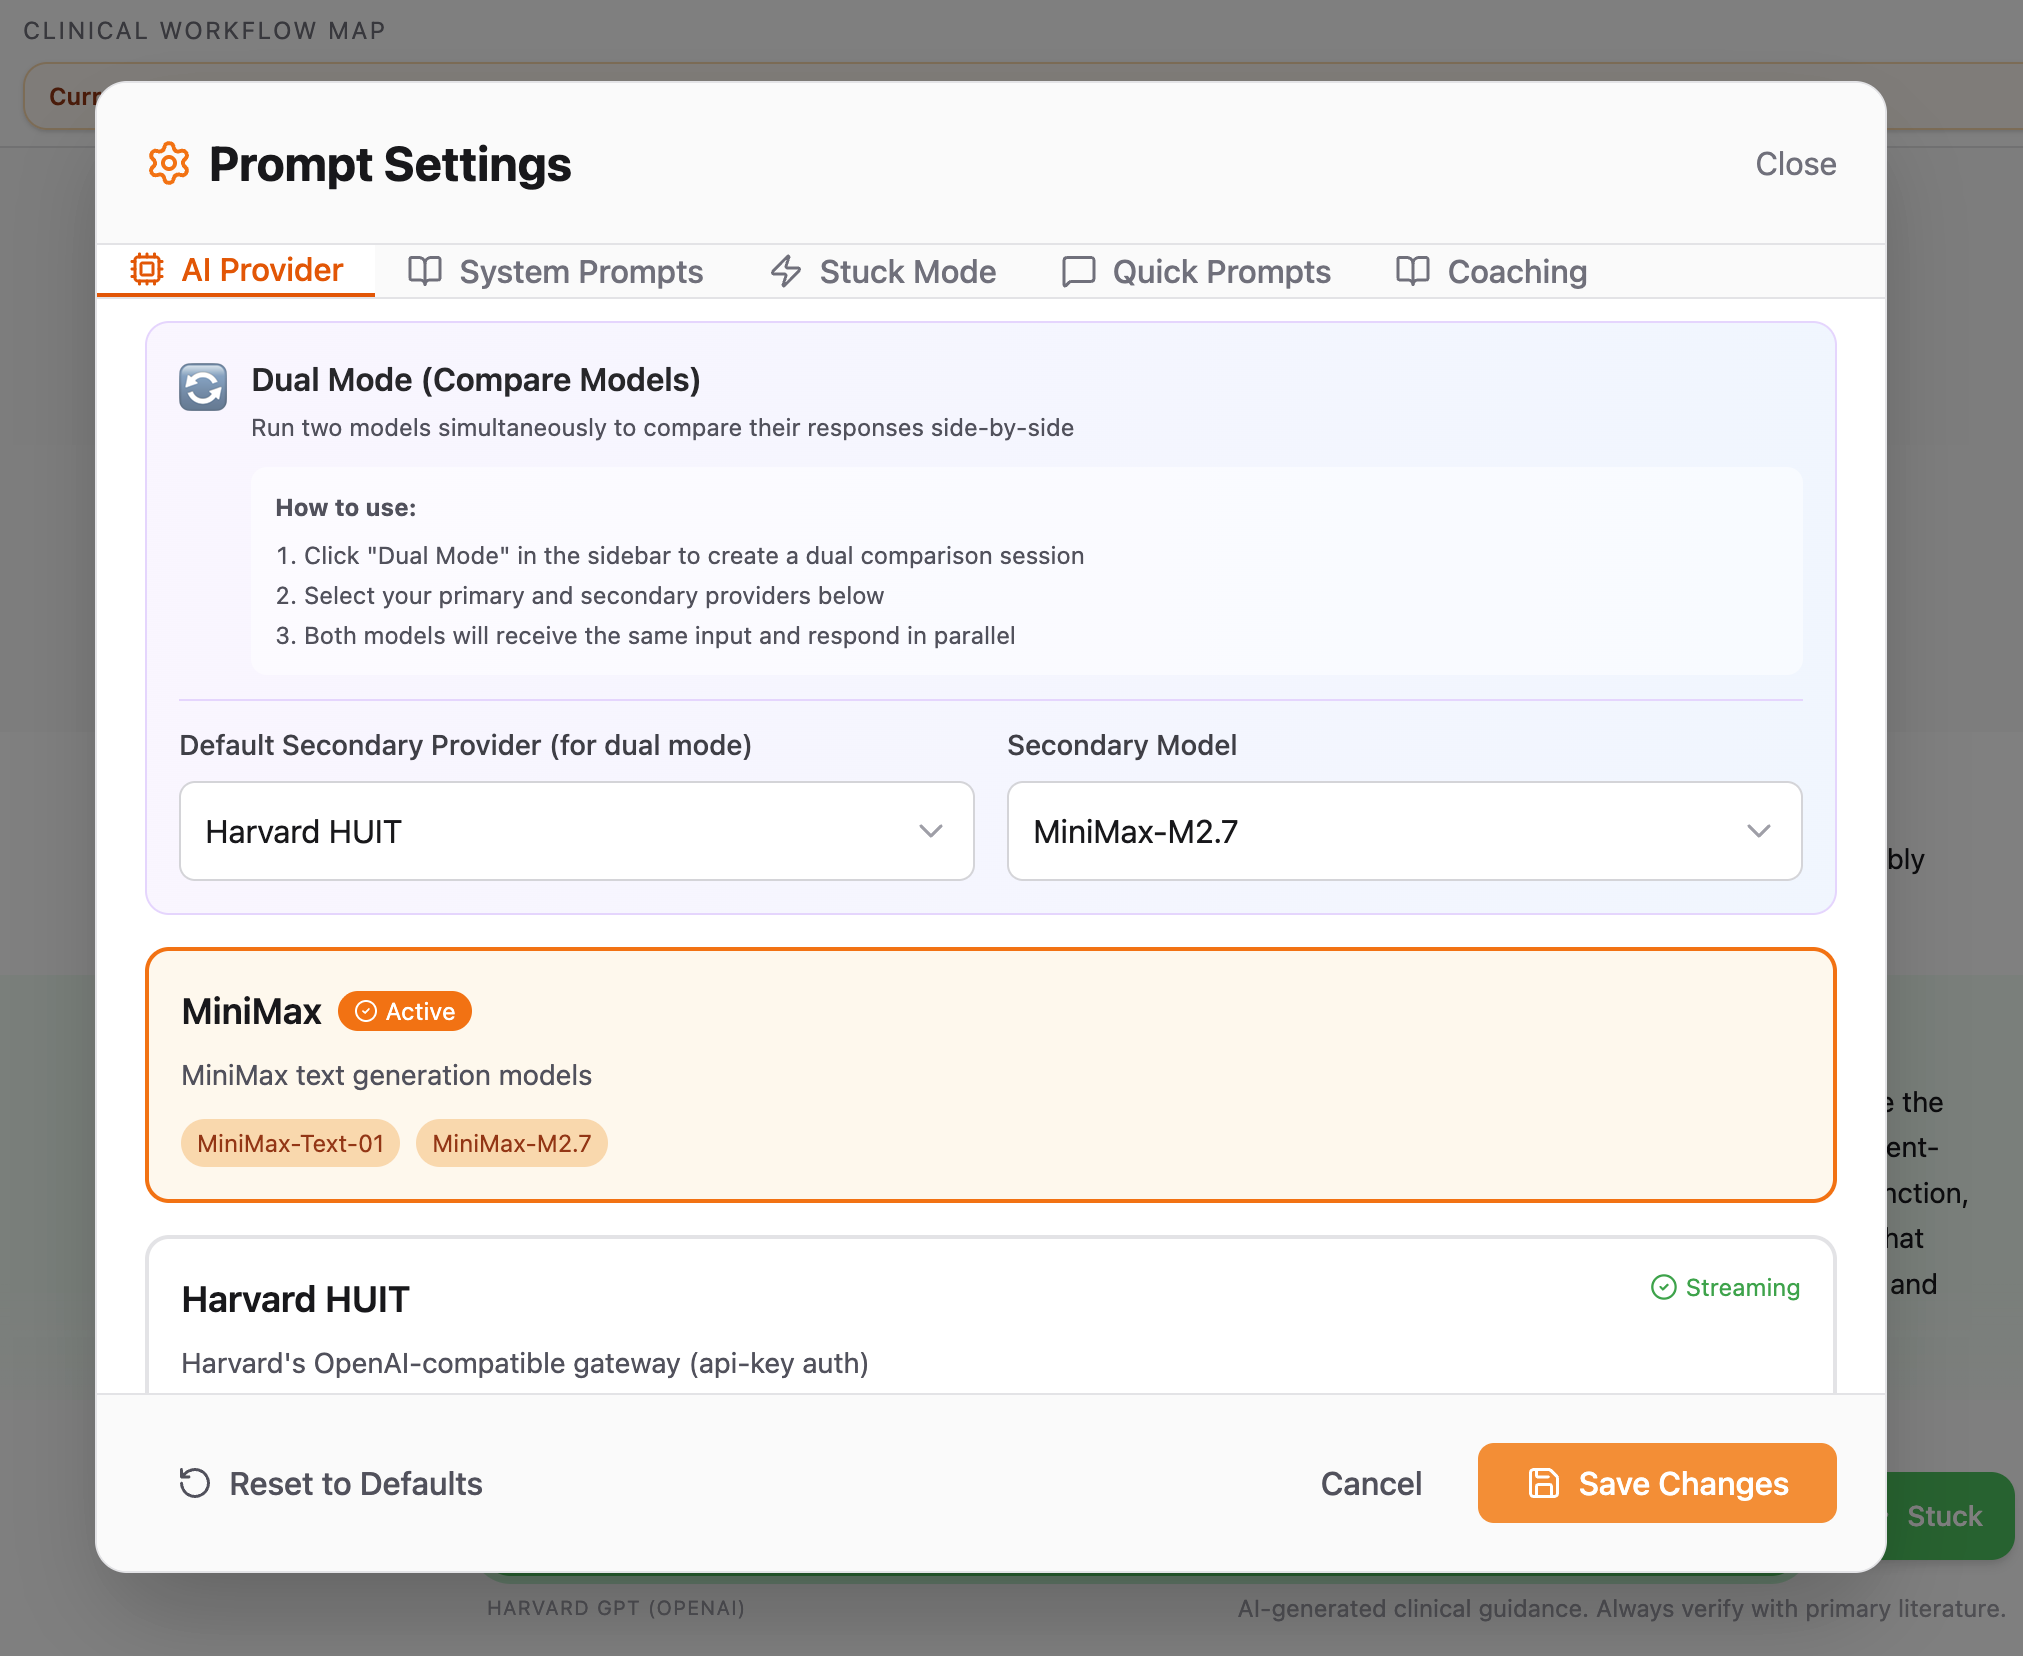
\includegraphics[width=0.75\textwidth]{figures/prompt_settings_provider.png}
    \caption{Settings dashboard for switching between LLM providers or activating Dual Mode evaluation.}
    \label{fig:provider_settings}
\end{figure}

The finding that a smaller mid-range model (Minimax M2.7) outperformed larger frontier models (GPT 5) in clinical communication tasks suggests that model selection should prioritize task-specific alignment over raw capability.

% ============================================================
\subsection{Navigation Map phase recognition shows non-deterministic variability}

This subsection addresses clinician feedback on the system's ability to correctly identify consultation phases within the Navigation Map framework.

Clinician feedback indicated that the system successfully provided appropriate communication advice and guidance. The language frameworks were correctly integrated by all tested models, and responses were formatted in the expected structure. Communication tools functioned as intended across consultation scenarios.

However, the non-deterministic nature of large language models presented challenges for Navigation Map phase recognition. Identical prompts could yield different phase assignments on repeated runs, as the system sometimes suggested alternative phases within the consultation journey. This variability was attributed to the inherently vague nature of dementia as a disease domain, which can be interpreted through multiple clinical perspectives.

Phase recognition variability was not evenly distributed:
\begin{itemize}
    \item Recognition and Diagnosis phases showed higher consistency
    \item Evaluation phase showed greater susceptibility to alternative interpretations
    \item Boundary cases between phases were most prone to non-deterministic assignment
\end{itemize}

The finding that phase recognition is sensitive to model randomness has implications for clinical deployment, where consistent phase identification may be important for tracking consultation progress.

\begin{figure}[h]
    \centering
    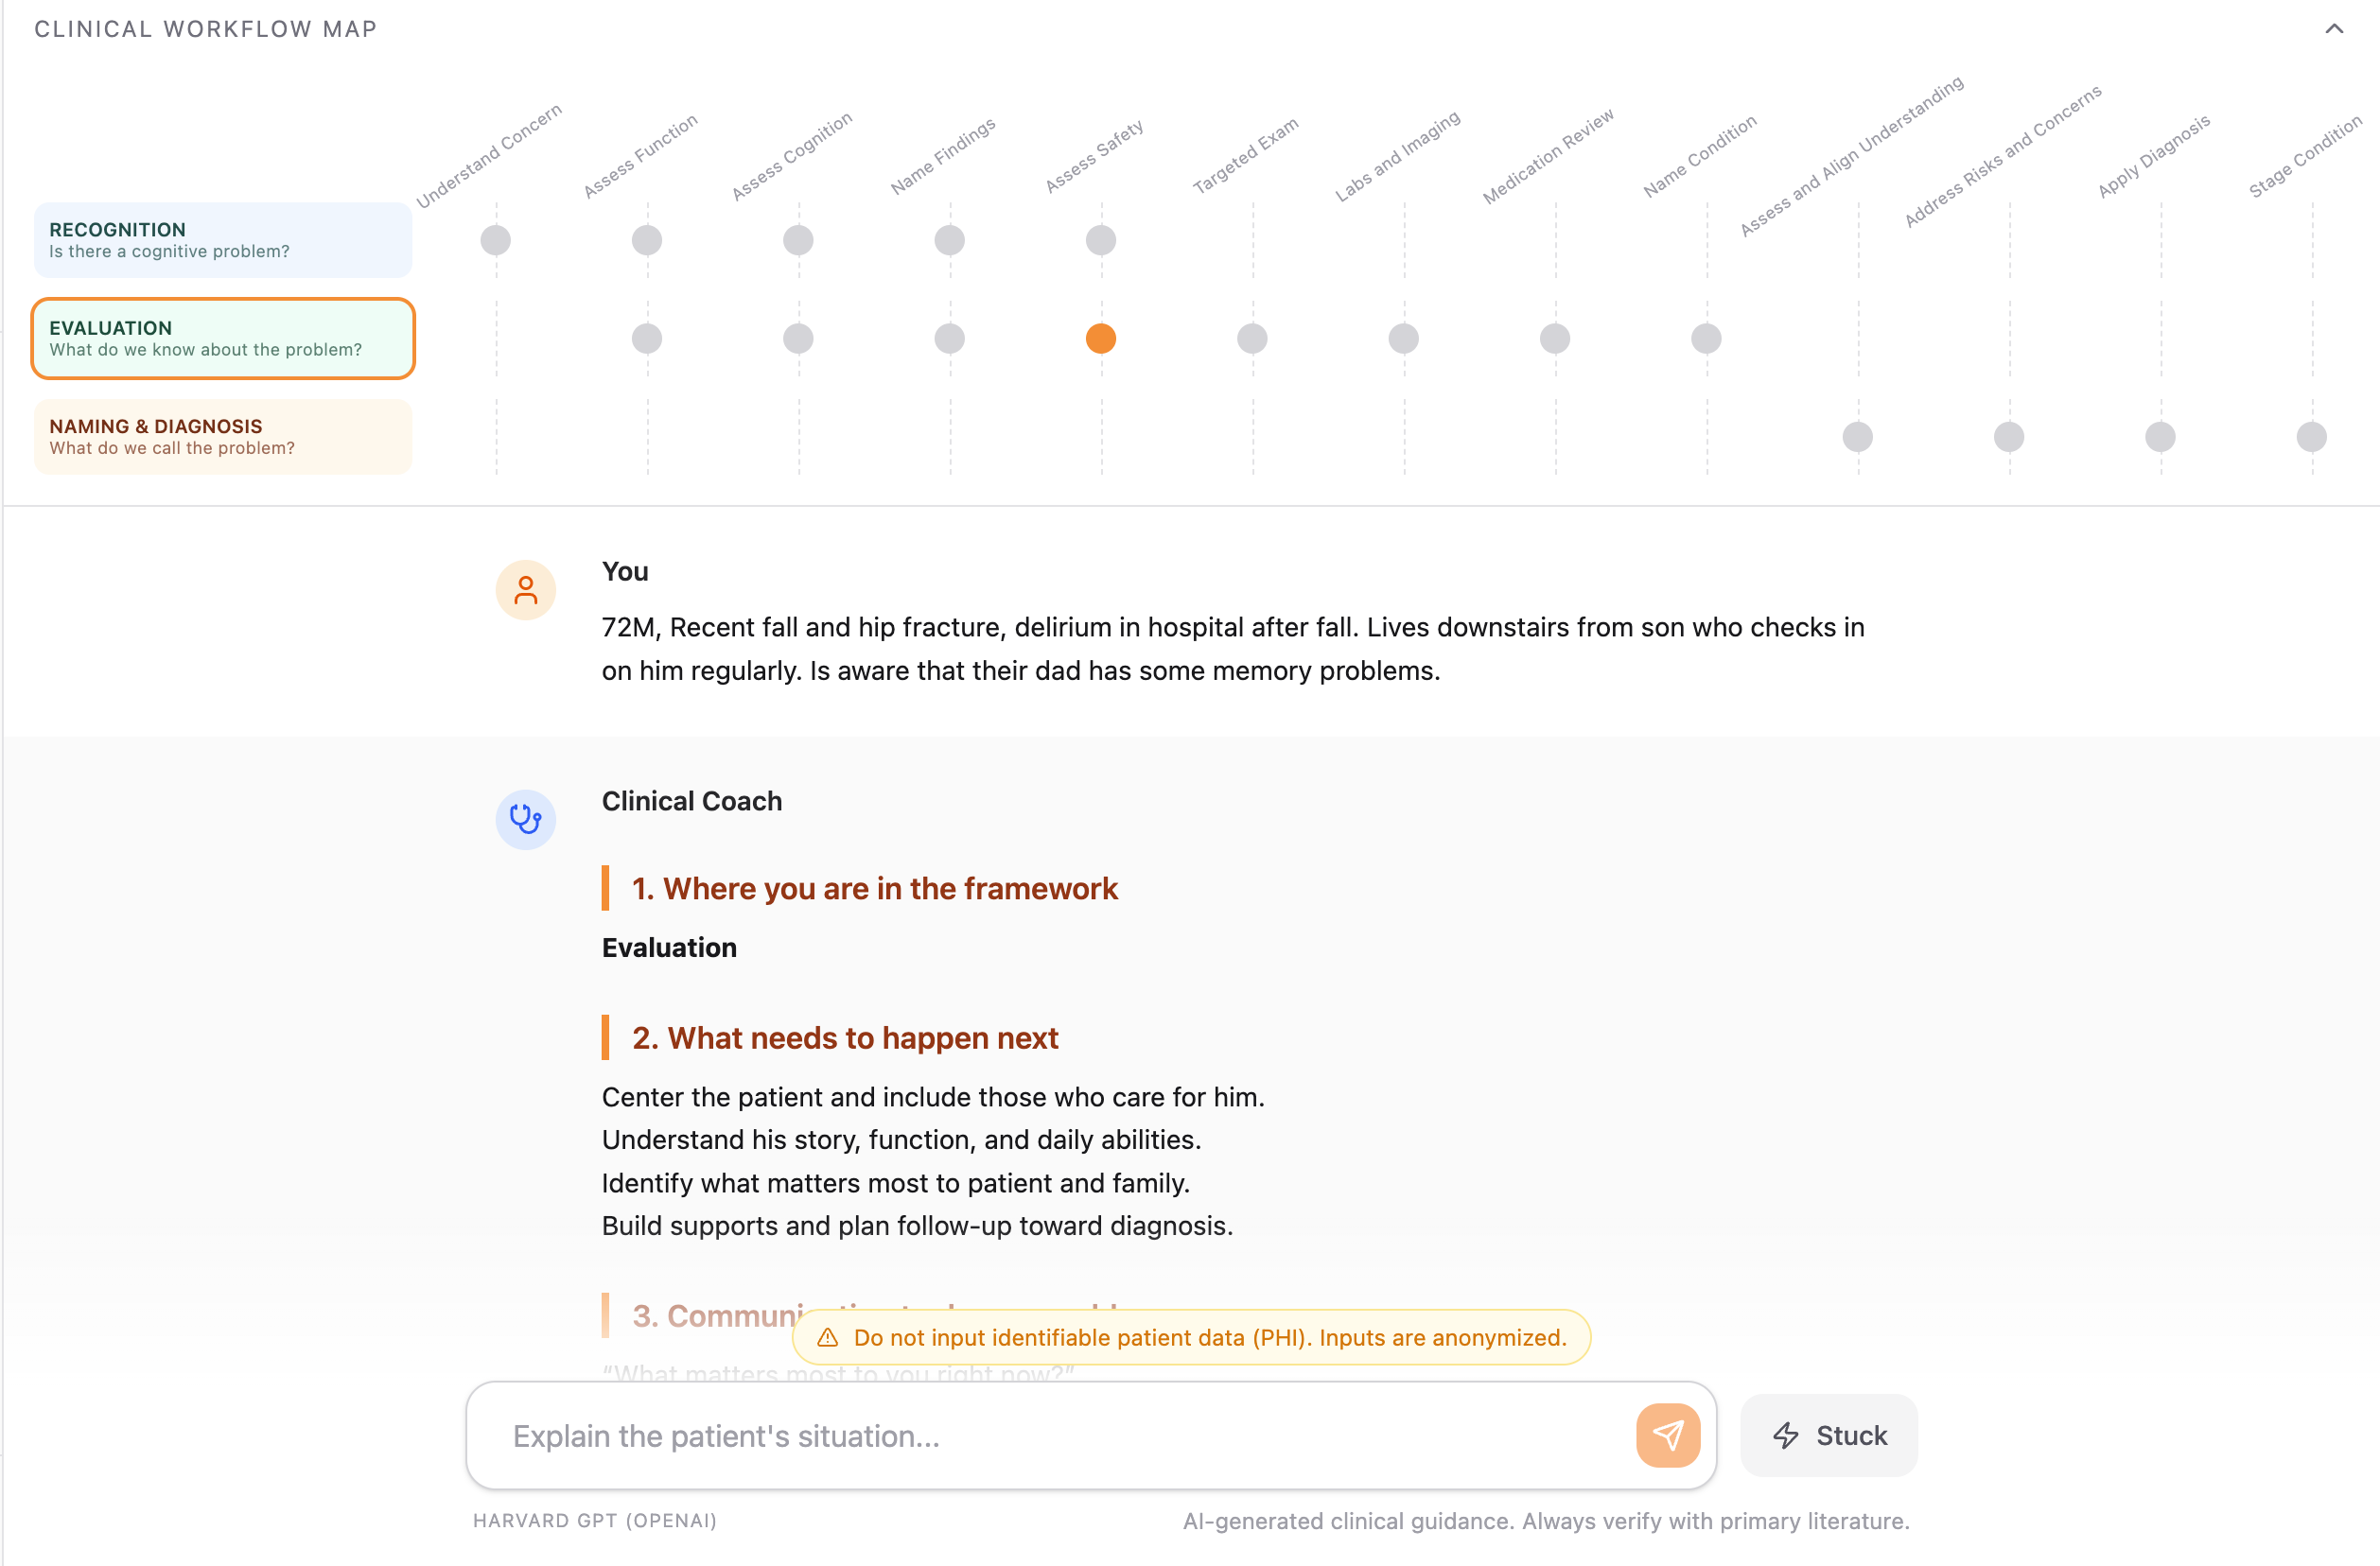
\includegraphics[width=0.85\textwidth]{figures/prompt_example.png}
    \caption{Example interaction showing structured response output with the Navigation Map highlighting the current consultation phase.}
    \label{fig:prompt_example}
\end{figure}

% ============================================================
\subsection{Stuck Points Framework appreciated for proactive guidance but requires UX refinement}

This subsection addresses clinician feedback on the Stuck Points Framework component of the consultation assistant.

The Stuck Points Framework received positive feedback from clinicians, particularly for its ability to identify and anticipate communication obstacles before they arose. Clinicians valued the system's proactive approach to smoothing clinical interactions by providing relational communication strategies in advance.

Specific positive feedback included:
\begin{itemize}
    \item Anticipatory identification of potential stuck points
    \item Language suggestions for navigating difficult moments
    \item Integration of emotional acknowledgment strategies
\end{itemize}

\begin{figure}[h]
    \centering
    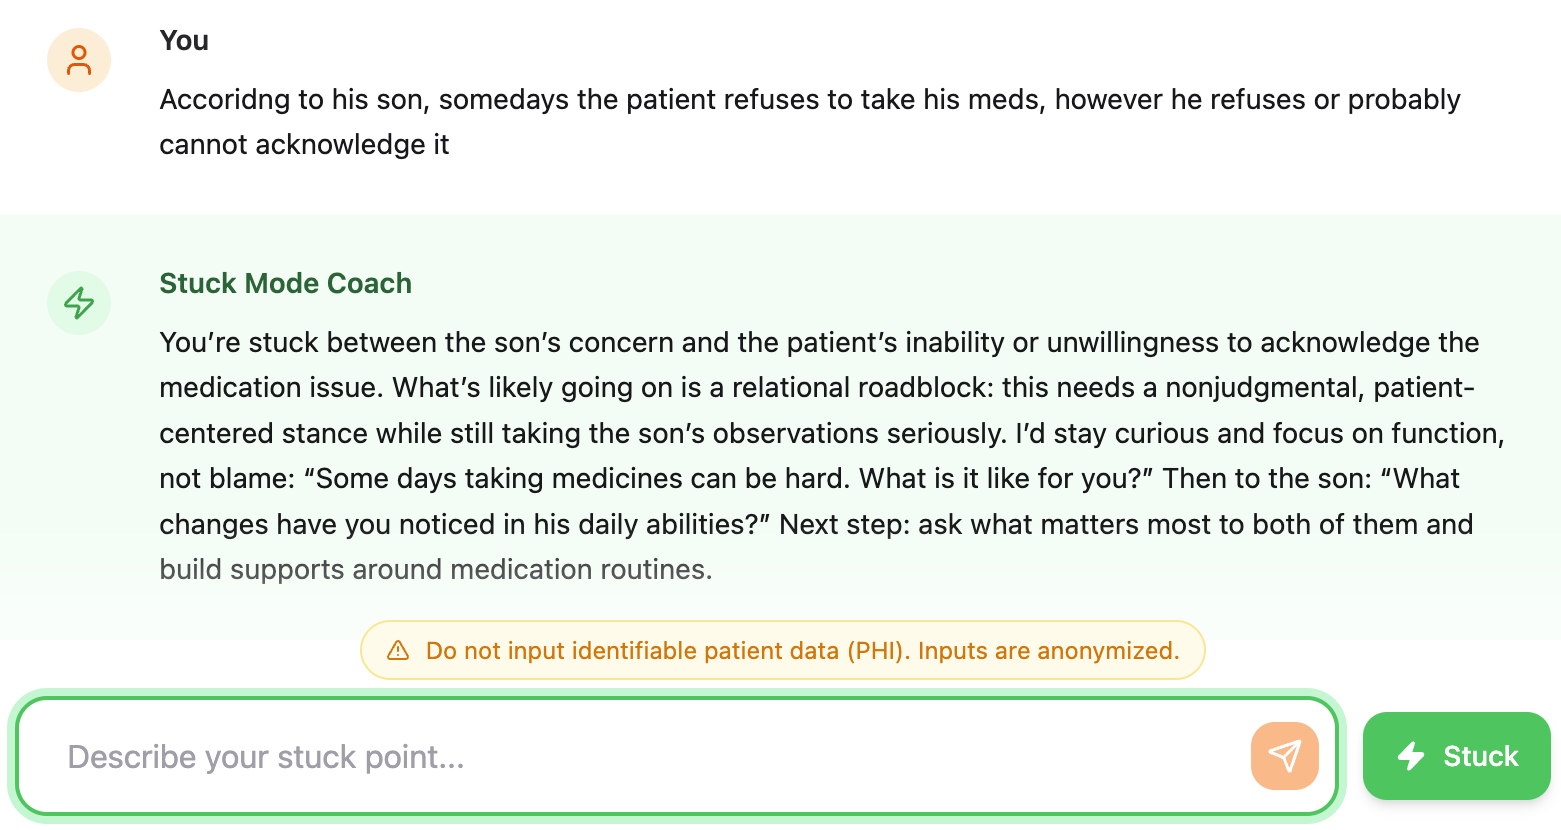
\includegraphics[width=0.85\textwidth]{figures/stuck_screenshot.png}
    \caption{Example output from the Stuck Points mode showing an input query and the system's relational communication guidance.}
    \label{fig:stuck_mode_example}
\end{figure}

However, clinicians noted that the standalone mode integration and user experience interface required refinement to optimize system-user interaction. Specific concerns included:
\begin{itemize}
    \item Navigation between primary guidance and Stuck Points modes
    \item Clarity of when Stuck Points suggestions were most relevant
    \item Overlap between main consultation guidance and relational support
\end{itemize}

The Stuck Points Framework demonstrated clinical utility but highlighted the importance of interface design in translating technical capability into practical workflow support.

% ============================================================